\documentclass[12pt]{report}
\usepackage{graphicx}
\usepackage{float}
\usepackage{lettrine}
\usepackage{caption}
\usepackage{url}
\usepackage[margin=1in]{geometry}
\usepackage{amsmath}
\usepackage{algorithm}
\usepackage[noend]{algpseudocode}
\usepackage{amssymb}

\newcommand\blfootnote[1]{%
  \begingroup
  \renewcommand\thefootnote{}\footnote{#1}%
  \addtocounter{footnote}{-1}%
  \endgroup
}

\title{Verification of GCD Circuits Using Algebraic Geometry}
\author{Jaden Simon - simonjaden223@gmail.com \\ \and
	   Daniel Humeniuk - d.humeniuk@utah.edu}

	   
\begin{document}

\maketitle

\section{Introduction}

The purpose of this report is to discuss our findings and results of our formal verification project for ECE 5745. Our original proposal was centered around verifying a 3-bit Elliptical Curve Arithmetic Unit (ECAU) circuit as a proof of concept. After some studying, our project led us to investigate the 3-bit greatest common divisor (GCD) circuit which would be required in a 3-bit ECAU. Our main point of investigation was to determine if verification of a 3-bit GCD circuit is trivial or nontrivial. Once this question could be answered, we could later explore if the verification could be easily transposed onto an $n$-bit GCD circuit.

This report will detail our findings as well as identified areas of further interest and exploration.

\section{Experiments and Test Setup}

Our first starting point was designing a circuit that computed a 3-bit GCD. This circuit can be seen in Figure \ref{fig:gcd}. Once this circuit was created, it took some refining to ensure that it would act as expected. A GCD circuit, as implemented here, would require at most $n$ clock cycles for an $n$-bit circuit. Once the circuit was created, we were then able to create polynomials for the nets in the circuits.

\begin{figure}
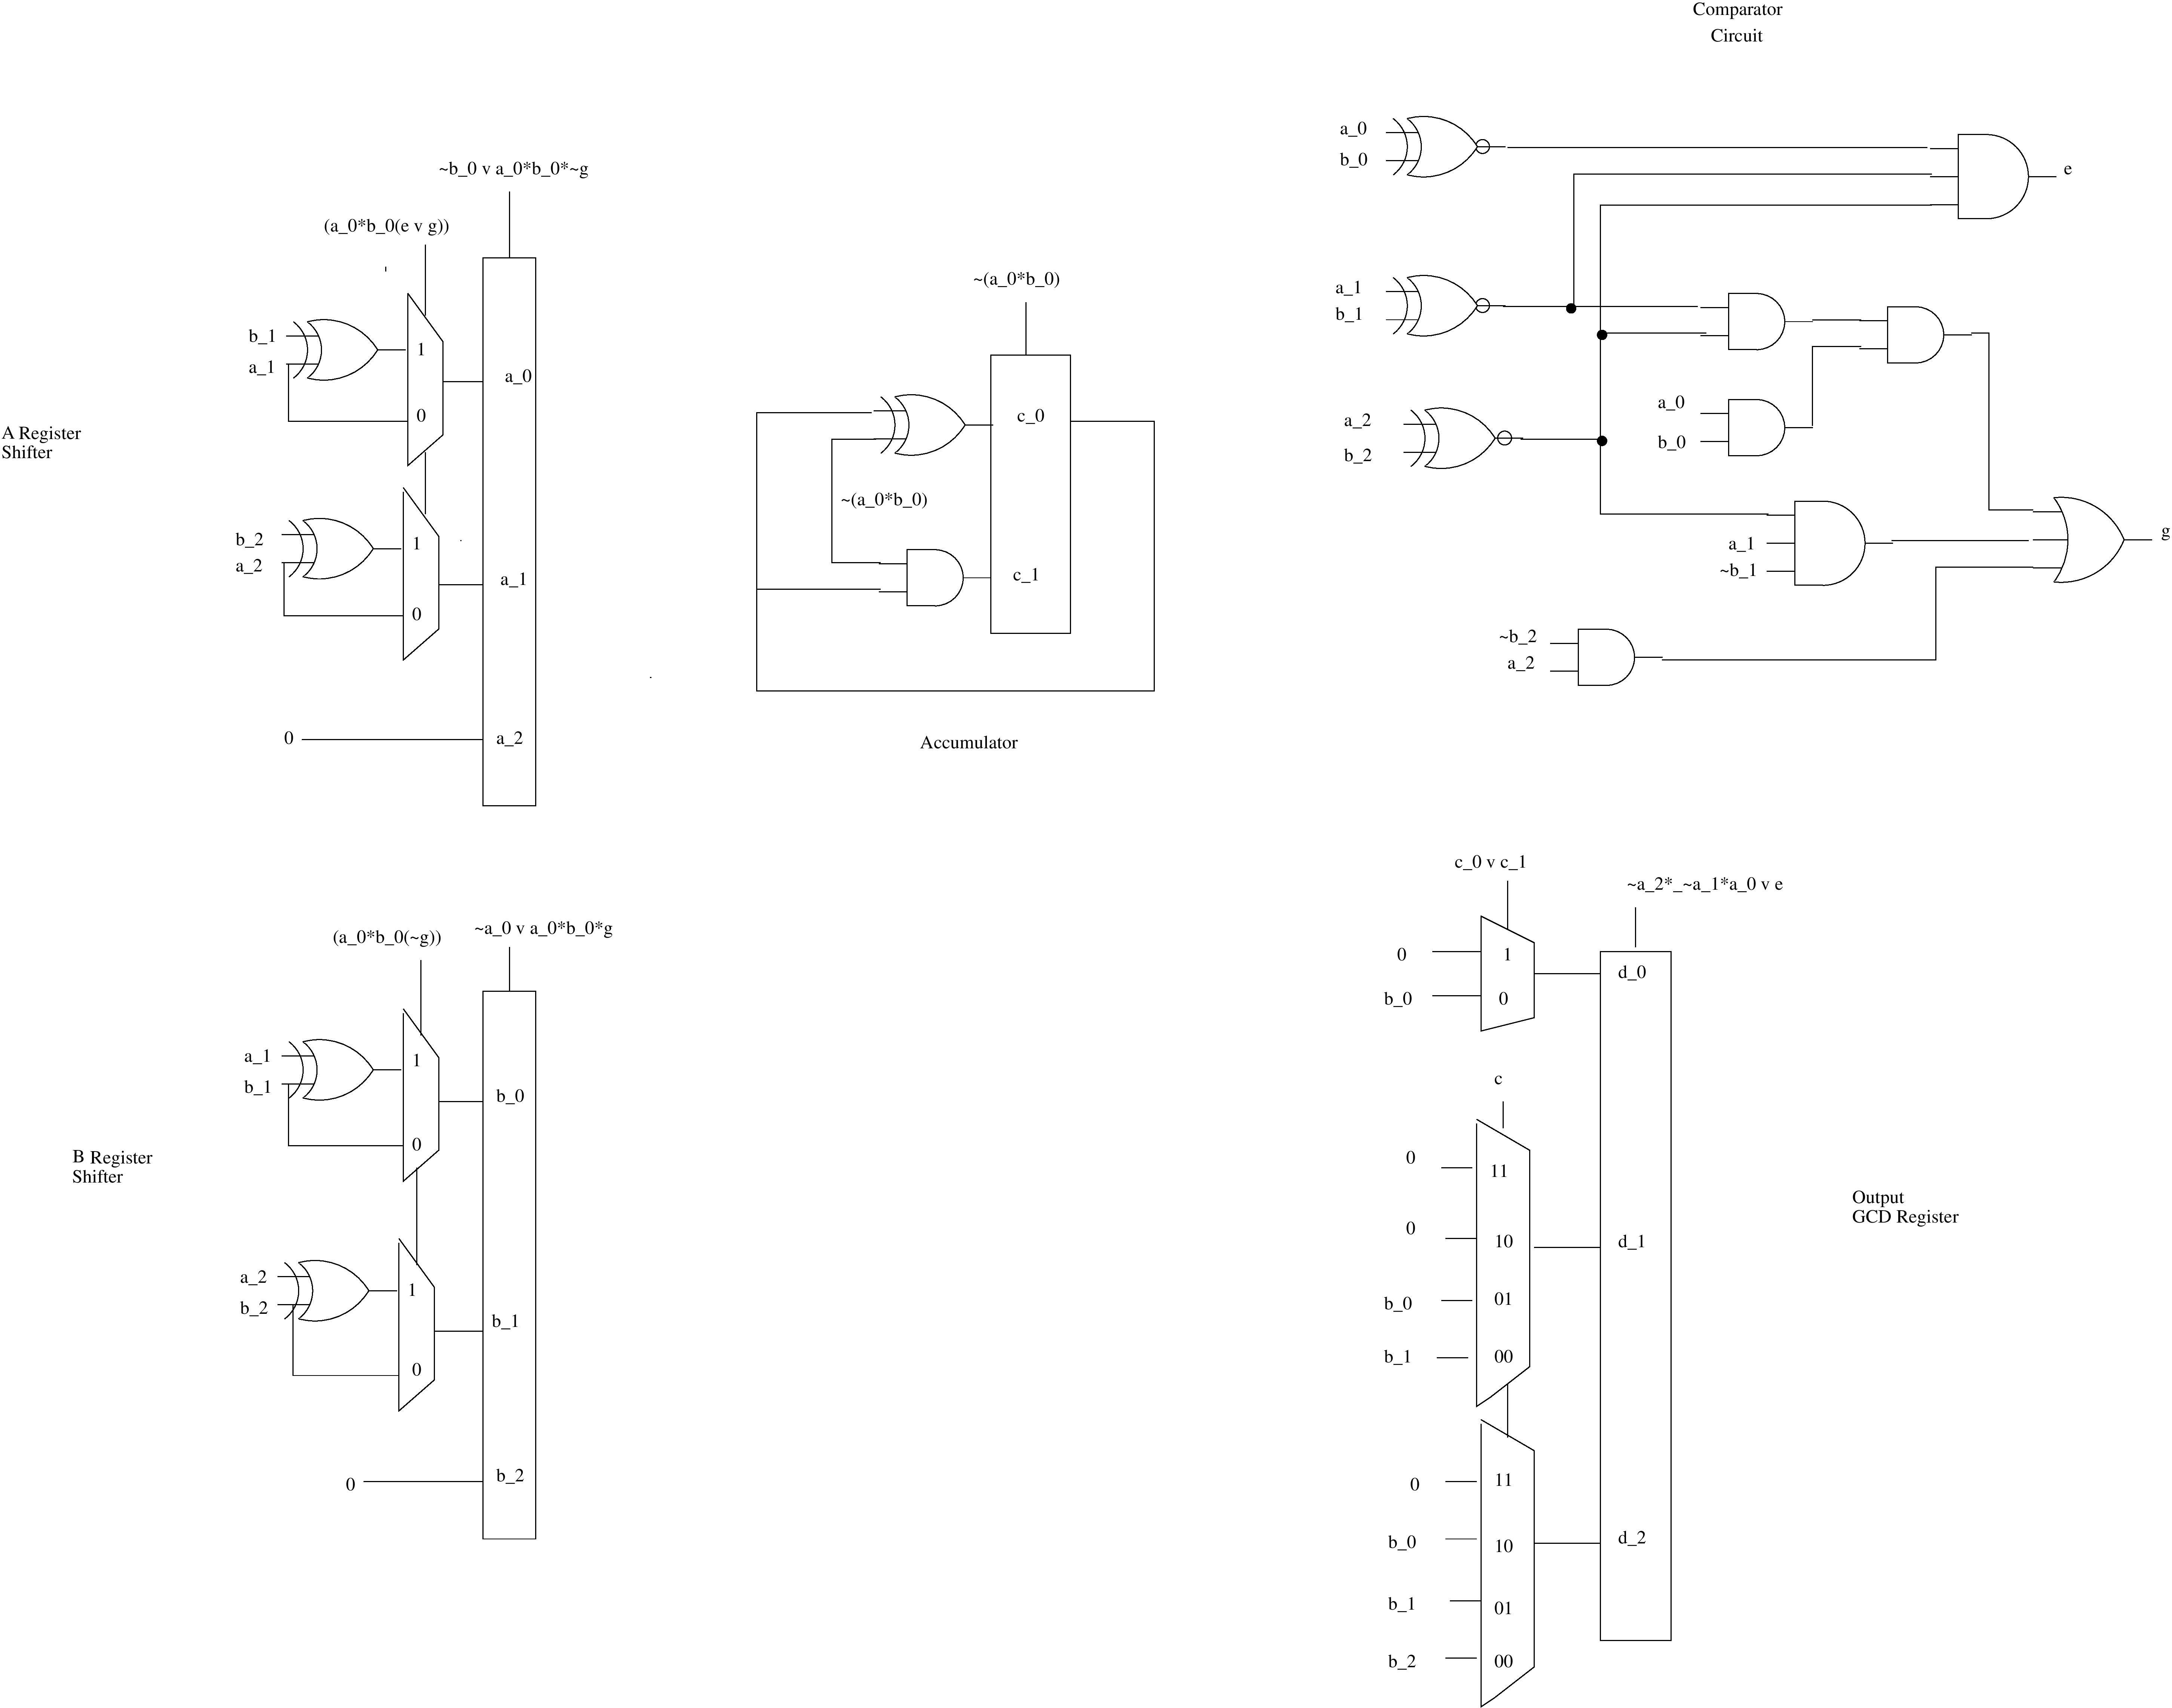
\includegraphics[scale=0.35]{images/gcd_page.png}
\caption{Binary GCD Algorithm for $3$ bits}
\label{fig:gcd}
\end{figure}

We first implemented the comparator circuit. The ring consisted of the primary inputs, the fan out branches, and the primary outputs. Once all of the polynomials were instantiated, an ideal J miter was used with each polynomial as well as the vanishing polynomials of the circuit. This aspect of the project is most likely trivial but worth while to ensure that our final implementation was correct. 

The GCD testing was conducted in similar fashion with the inputs, outputs, and nets of the circuit being instantiated into polynomials. There was a great deal of polynomials required for such a circuit. This process will need to be automated when dealing with circuits larger than 3 bits. One of the difficulties in the process was learning how to write a multiplexer as a polynomial. Once discovered, it still became an annoyance but was easier than doing a multiplexer as a series of AND and Inverter gates. Once each circuit block was completed, we created a very long list of vanishing polynomials. Once the ideal was created, a Groebner basis was created using the $slimgb$ function in Singular. From here, we were able to determine the output D and the next states for inputs A and B. 

For our implementation in the Singular file, we only wanted to see what the circuit would output as the next state and not the final output for D. D will output 0 iff the circuit has not found the GCD of the two inputs A and B. Once the conditions for output D were satisfied, an output other than 0 would be present. We implemented it this way because we wanted to see the next states of A and B as well and not run through all of the cycles required for the circuit. 

Getting the circuit to work over the field $\mathbb{Q}$ did not prove to be fruitful. There were issues that are far too tedious to fix for such a short time frame. More study will be required if such verification were to be performed. 

\section{Findings}

Our first finding was very interesting. When we were performing the verification, we were conducting the experiment over a finite field. This resulted in our discovery verification for this particular circuit would not work over a finite field as every element within a finite field divides every other element. Our circuit could have been simplified to returning either A or B as either one divides the other. To verify the circuit as it is working as we intended, we needed to add a subtraction component to the circuit.

\section{Conclusion}

The verification of the GCD circuit proved to be a very interesting project to work on. More research will need to be conducted to determine the exact nature of the problem. There also remains the question of the use of a GCD circuit in real world applications. If an ECAU was implemented in hardware, it is unlikely that a GCD component would be used as other techniques are used to find the inverse of a given integer. The study of verifying a GCD is interesting but may not be as applicable in real world applications.

\bibliographystyle{IEEEtran}

%\bibliography{IEEEabrv,bib/ref}

\end{document}